经过生物滴滤池15d的稳定运行后,在温度为25-30℃,循环液pH值控制在6.5-7.0,气流量为9000m3/h的条件下,生物滤池对的氨及硫化氢的降解效果如下图。\par
{\noindent  \centering  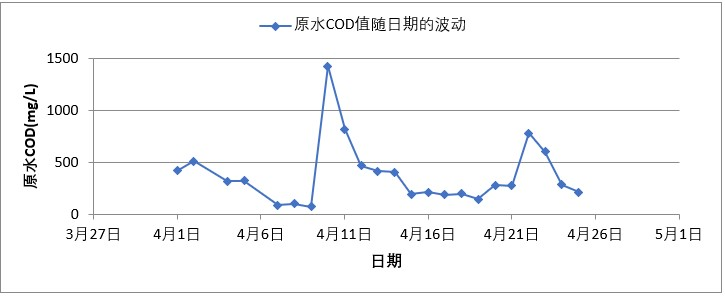
\includegraphics[width=150mm]{Img/fig1.jpg}\par}
{\hspace{40mm} 
图1 氨的进、出气浓度及去除率}
\vspace{10mm}
\par
{\noindent    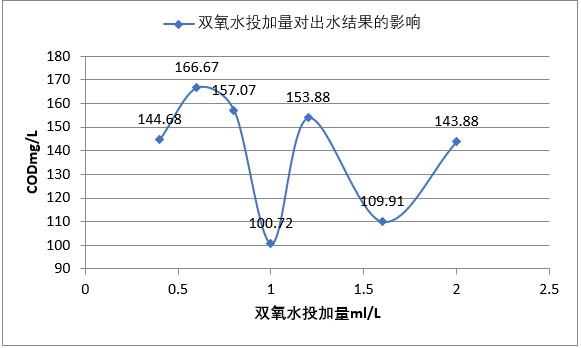
\includegraphics[width=150mm]{Img/fig2.jpg}\par}
{\hspace{40mm} 图2 硫化氢的进、出气浓度及去除率}\par
\vspace{10mm}
通过实验得出:在氨氮及硫化氢浓度在100ppmv以下,用生物滴滤池处理城市污水处理厂臭气运行效果良好。\par
